%%%%%%%%%%%%%%%%%%%%%%%%%%%%%%%%%%%%%%%%%%%%%%%%%%%%%%%%%%%%%%%%%%%%%%%%%%%%%%%%%%%%%%%%%%%%%%%%%%%%%%%%%%%%%%%%%%%%%%%%%%%%%%%%%%%%%%%%%%%%%%%%%%%%%%%%%%%
% This is just an example/guide for you to refer to when submitting manuscripts to Frontiers, it is not mandatory to use Frontiers .cls files nor frontiers.tex  %
% This will only generate the Manuscript, the final article will be typeset by Frontiers after acceptance.   
%                                              %
%                                                                                                                                                         %
% When submitting your files, remember to upload this *tex file, the pdf generated with it, the *bib file (if bibliography is not within the *tex) and all the figures.
%%%%%%%%%%%%%%%%%%%%%%%%%%%%%%%%%%%%%%%%%%%%%%%%%%%%%%%%%%%%%%%%%%%%%%%%%%%%%%%%%%%%%%%%%%%%%%%%%%%%%%%%%%%%%%%%%%%%%%%%%%%%%%%%%%%%%%%%%%%%%%%%%%%%%%%%%%%

%%% Version 3.4 Generated 2018/06/15 %%%
%%% You will need to have the following packages installed: datetime, fmtcount, etoolbox, fcprefix, which are normally inlcuded in WinEdt. %%%
%%% In http://www.ctan.org/ you can find the packages and how to install them, if necessary. %%%
%%%  NB logo1.jpg is required in the path in order to correctly compile front page header %%%

\documentclass[utf8]{frontiersSCNS} % for Science, Engineering and Humanities and Social Sciences articles
%\documentclass[utf8]{frontiersHLTH} % for Health articles
%\documentclass[utf8]{frontiersFPHY} % for Physics and Applied Mathematics and Statistics articles

%\setcitestyle{square} % for Physics and Applied Mathematics and Statistics articles
\usepackage{url,hyperref,lineno,microtype,subcaption}
\usepackage[onehalfspacing]{setspace}

\usepackage{color}
\usepackage{fancyvrb}
\newcommand{\VerbBar}{|}
\newcommand{\VERB}{\Verb[commandchars=\\\{\}]}
\DefineVerbatimEnvironment{Highlighting}{Verbatim}{commandchars=\\\{\}}
% Add ',fontsize=\small' for more characters per line
\usepackage{framed}
\definecolor{shadecolor}{RGB}{248,248,248}
\newenvironment{Shaded}{\begin{snugshade}}{\end{snugshade}}
\newcommand{\KeywordTok}[1]{\textcolor[rgb]{0.13,0.29,0.53}{\textbf{{#1}}}}
\newcommand{\DataTypeTok}[1]{\textcolor[rgb]{0.13,0.29,0.53}{{#1}}}
\newcommand{\DecValTok}[1]{\textcolor[rgb]{0.00,0.00,0.81}{{#1}}}
\newcommand{\BaseNTok}[1]{\textcolor[rgb]{0.00,0.00,0.81}{{#1}}}
\newcommand{\FloatTok}[1]{\textcolor[rgb]{0.00,0.00,0.81}{{#1}}}
\newcommand{\CharTok}[1]{\textcolor[rgb]{0.31,0.60,0.02}{{#1}}}
\newcommand{\StringTok}[1]{\textcolor[rgb]{0.31,0.60,0.02}{{#1}}}
\newcommand{\CommentTok}[1]{\textcolor[rgb]{0.56,0.35,0.01}{\textit{{#1}}}}
\newcommand{\OtherTok}[1]{\textcolor[rgb]{0.56,0.35,0.01}{{#1}}}
\newcommand{\AlertTok}[1]{\textcolor[rgb]{0.94,0.16,0.16}{{#1}}}
\newcommand{\FunctionTok}[1]{\textcolor[rgb]{0.00,0.00,0.00}{{#1}}}
\newcommand{\RegionMarkerTok}[1]{{#1}}
\newcommand{\ErrorTok}[1]{\textbf{{#1}}}
\newcommand{\NormalTok}[1]{{#1}}
\usepackage{graphicx}
% Redefine \includegraphics so that, unless explicit options are
% given, the image width will not exceed the width of the page.
% Images get their normal width if they fit onto the page, but
% are scaled down if they would overflow the margins.
\makeatletter
\def\ScaleIfNeeded{%
  \ifdim\Gin@nat@width>\linewidth
    \linewidth
  \else
    \Gin@nat@width
  \fi
}
\makeatother
\let\Oldincludegraphics\includegraphics
{%
 \catcode`\@=11\relax%
 \gdef\includegraphics{\@ifnextchar[{\Oldincludegraphics}{\Oldincludegraphics[width=\ScaleIfNeeded]}}%
}%

\linenumbers


% Leave a blank line between paragraphs instead of using \\


\def\keyFont{\fontsize{8}{11}\helveticabold }
\def\firstAuthorLast{Sample {et~al.}} %use et al only if is more than 1 author
\def\Authors{First Author}
% Affiliations should be keyed to the author's name with superscript numbers and be listed as follows: Laboratory, Institute, Department, Organization, City, State abbreviation (USA, Canada, Australia), and Country (without detailed address information such as city zip codes or street names).
% If one of the authors has a change of address, list the new address below the correspondence details using a superscript symbol and use the same symbol to indicate the author in the author list.
\def\Address{Address}
% The Corresponding Author should be marked with an asterisk
% Provide the exact contact address (this time including street name and city zip code) and email of the corresponding author
\def\corrAuthor{Corresponding Author}

\def\corrEmail{email@uni.edu}




\begin{document}
\onecolumn
\firstpage{1}

\title[Running Title]{Demo Manuscript} 

\author[\firstAuthorLast ]{\Authors} %This field will be automatically populated
\address{} %This field will be automatically populated
\correspondance{} %This field will be automatically populated

\extraAuth{}% If there are more than 1 corresponding author, comment this line and uncomment the next one.
%\extraAuth{corresponding Author2 \\ Laboratory X2, Institute X2, Department X2, Organization X2, Street X2, City X2 , State XX2 (only USA, Canada and Australia), Zip Code2, X2 Country X2, email2@uni2.edu}


\maketitle


\begin{abstract}

Hello, this is the abstract.

  \tiny
   \keyFont{ \section{Keywords:} keyword1, kw2, kw3\ldots{} have to have at least 5, max 8} %All article types: you may provide up to 8 keywords; at least 5 are mandatory.

\end{abstract}

Hello, world!

\section{Introduction}\label{introduction}

Here are some things to consider:

\begin{enumerate}
\def\labelenumi{\arabic{enumi}.}
\itemsep1pt\parskip0pt\parsep0pt
\item
  We don't know what's happening
\item
  Neither does anyone else
\end{enumerate}

Also important:

\begin{itemize}
\itemsep1pt\parskip0pt\parsep0pt
\item
  this creates an unordered list
\item
  and this is the second item.
\end{itemize}

This is how links work: \href{https://example.com/}{link text}

We can also include code snippets:

\begin{Shaded}
\begin{Highlighting}[]
\CommentTok{# Examplary python code}
\DataTypeTok{print}\NormalTok{(}\StringTok{"Hello World!"}\NormalTok{)}
\DataTypeTok{print}\NormalTok{(}\StringTok{"2 + 5 = "} \NormalTok{+ (}\DecValTok{2+5}\NormalTok{))}
\KeywordTok{with} \DataTypeTok{open}\NormalTok{(}\StringTok{'testfile.fa'}\NormalTok{, }\StringTok{'w'}\NormalTok{) }\CharTok{as} \DataTypeTok{file}\NormalTok{:}
  \DataTypeTok{file}\NormalTok{.write(}\StringTok{"Hello, world"}\NormalTok{)}
\DataTypeTok{print}\NormalTok{(}\StringTok{"Done"}\NormalTok{)}
\end{Highlighting}
\end{Shaded}

\section{Rmarkdown}\label{rmarkdown}

Now for some really kewl stuff: We load a file in R:

\begin{Shaded}
\begin{Highlighting}[]
\NormalTok{annotation_quantities =}\StringTok{ }
\StringTok{  }\KeywordTok{read.csv}\NormalTok{(}\StringTok{'../../../data/mocks/processed/annotation_quantities.csv'}\NormalTok{, }\DataTypeTok{header=}\NormalTok{T)}
\NormalTok{rice =}\StringTok{ }\KeywordTok{subset}\NormalTok{(annotation_quantities, genome==}\StringTok{'rice'} \NormalTok{&}\StringTok{ }\NormalTok{source==}\StringTok{'GOMAP'}\NormalTok{)}
\end{Highlighting}
\end{Shaded}

And now we can actually use it:

\begin{Shaded}
\begin{Highlighting}[]
\KeywordTok{head}\NormalTok{(annotation_quantities)}
\end{Highlighting}
\end{Shaded}

\begin{verbatim}
##     genome    source n_c n_f n_p n_genes
## 1 maize_v3     GOMAP  95  56 169      11
## 2 maize_v3 Gramene49  63  83  74      11
## 3 maize_v3 Phytozome  14  67  59      11
## 4 maize_v4     GOMAP  52  65 213      11
## 5     rice     GOMAP  60  67 223      11
\end{verbatim}

\begin{Shaded}
\begin{Highlighting}[]
\KeywordTok{summary}\NormalTok{(annotation_quantities$n_c)}
\end{Highlighting}
\end{Shaded}

\begin{verbatim}
##    Min. 1st Qu.  Median    Mean 3rd Qu.    Max. 
##    14.0    52.0    60.0    56.8    63.0    95.0
\end{verbatim}

The annotation set for rice had a total of 60 annotations for cellular
component.

\subsection{Plots}\label{plots}

We can even plot the data:

\begin{Shaded}
\begin{Highlighting}[]
\NormalTok{a =}\StringTok{ }\NormalTok{annotation_quantities}
\KeywordTok{pie}\NormalTok{(a$n_c+a$n_f+a$n_p, }\DataTypeTok{labels=}\KeywordTok{paste}\NormalTok{(a$genome, a$source))}
\end{Highlighting}
\end{Shaded}

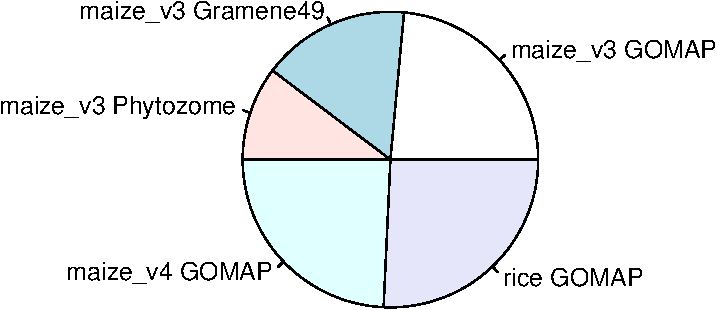
\includegraphics{demo-manuscript_files/figure-latex/plot-1.pdf}

\begin{Shaded}
\begin{Highlighting}[]
\KeywordTok{barplot}\NormalTok{(a$n_c+a$n_f+a$n_p, }\DataTypeTok{las=}\DecValTok{2}\NormalTok{)}
\end{Highlighting}
\end{Shaded}

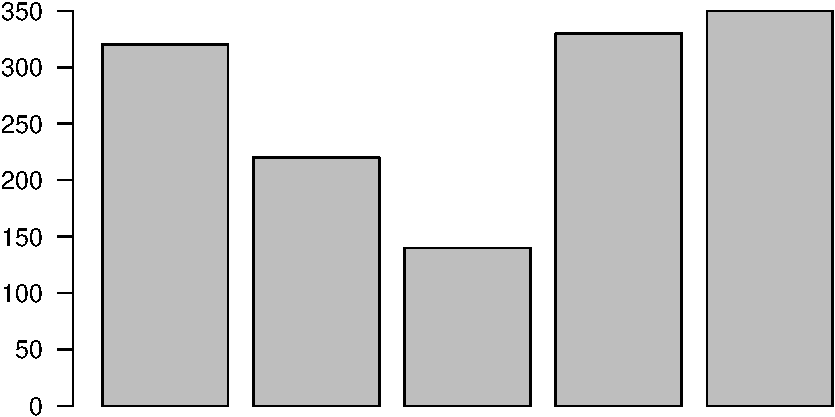
\includegraphics{demo-manuscript_files/figure-latex/plot2-1.pdf}

Now here is an actual figure I've been working on:

\begin{figure}[htbp]
\centering
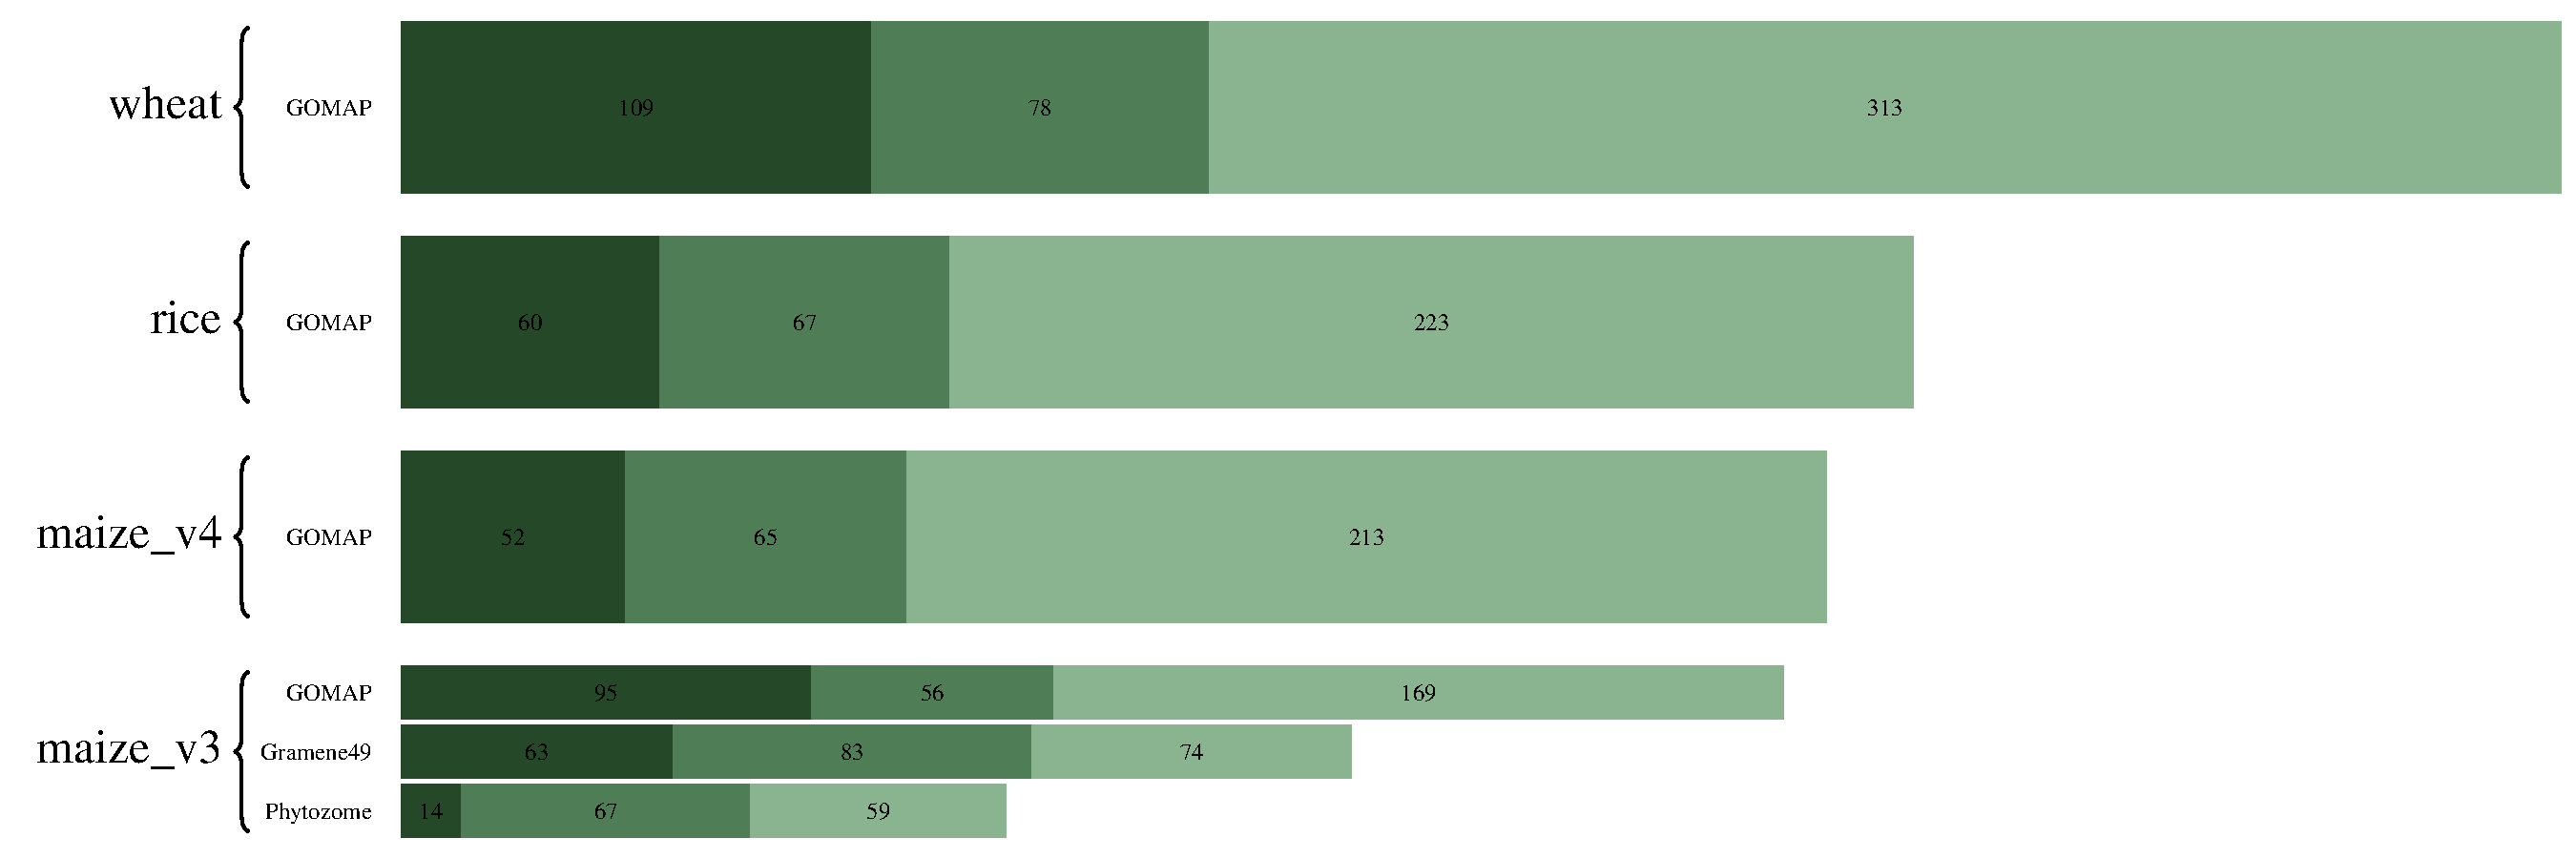
\includegraphics{../../../reports/figures/annotation_quantities.pdf}
\caption{Quantitiative lalala}
\end{figure}

\end{document}
